\documentclass{ECOS_2019}
\makeatletter
\let\NAT@parse\undefined
\makeatother
\makenomenclature
\usepackage{etoolbox}
\renewcommand\nomgroup[1]{%
  \item[\bfseries
  \ifstrequal{#1}{S}{Set and indices}{%
  \ifstrequal{#1}{P}{Parameters}{%
  \ifstrequal{#1}{V}{Variables}{%
  \ifstrequal{#1}{F}{Functions}{}}}}%
]}

\title{Assessment of a Parabolic dish-Stirling-Diesel-battery system for rural electrification in Bolivia}

\author{Pablo Jimenez Zabalaga$^{a}$, Sergio Balderrama$^{a,b}$, Evelyn Cardozo$^{a}$, Ioannis Boukas$^{c}$}

\address{$^{a}$ San Simon University, Centro Universitario de Investigacion en Energia,
Cochabamba,
Bolivia,
p.jimenez@umss.edu.bo
\and
$^{b}$ University of Liège, Energy System Research Unit - Thermodynamics Laboratory, Department of Mechanical and Aerospace Engineering,
Liège,
Belgium,
slbalderrama@doct.uliege.be
\and
$^{c}$ University of Liège, Department of Electrical Engineering and Computer Science,
Liège,
Belgium,
ioannis.boukas@uliege.be}

\abstract{In the last decades, the growing energy demand, variable price of fossil fuels, depletion of oil resources and progressive concerns about increasing greenhouse gas emissions have been encouraging the development of affordable, sustainable and reliable technologies for power generation. Nowadays, the Bolivian energy matrix relies largely (95\%) on fossil fuels. Moreover, almost all diesel, gasoline and other petroleum products supplies are imported and subsidized by the state. In this context, the government has been promoting projects that boost the energy transition of the country towards distributed renewable generation. Thus, the design, construction and control of hybrid microgrids constitutes an important component towards this goal. In this paper, a novel hybrid microgrid that relies on renewable generation technologies is proposed and techno-economically assessed using different control strategies. The proposed system is composed of a concentrated parabolic solar dish, a Stirling engine and a diesel generator, integrated with a bidirectional inverter and a battery bank. In this way, the novelty of the study relies on replacing conventional isolated systems, such as a typical diesel and battery assembly, with a system that is composed of a parabolic dish Stirling engine in combination with a small diesel generator and a battery. It is demonstrated that the latter system has the potential to achieve higher efficiency and economic feasibility. The parabolic solar dish Stirling (PSDS) engine serves as the primary source of electricity generation while the diesel generator in conjunction with the battery bank provides electrical energy backup when the primary source of power is unavailable. A model of the PSDS is used in combination with an open-source simulator of the microgrid operation. The developed model is used to study an hypothetical case of electrification for a 100-household rural village in Bolivia called Pojo Pata. The performance of the PSDS microgrid is tested using different control techniques (e.g., rule-based controller, optimization-based controller). The results indicate that the proposed system is very competitive compared to other renewable energy technologies such as photovoltaic panels. Whereas PV-Diesel-battery system still had a lower levelized cost of electricity (LCOE) and operational cost than the studied system, the PSDS microgrid can represent about 16\% of savings in terms of LCOE and 21\% of operational savings in comparison to the conventional Diesel-battery system. The paper could be found in Github repository under the following link: \href{https://github.com/pabloadolfo24/proyecto_final.git}{pabloadolfo24/proyecto\_final.git}}

\keywords{Microgrid, Parabolic solar dish, Stirling engine, Diesel genset, Batteries.}

\begin{document}
\newpage
\section{INTRODUCTION}
The role of electricity is fundamental for the economic and social development of a community as it has become a support for daily human activities. An increase in the rate of electricity access enhances the opportunities for industrial development and improves the quality of health and education services\cite{WorldBank}. During the last decades, the growing energy demand, variable price of fossil fuels, depletion of oil resources and progressive concern about greenhouse gas emissions have promoted the development of clean and efficient technologies for energy generation\cite{Essa2020,Salehi2020,Wies2012}.\\
In this context, United Nations (UN) have established the access to affordable, reliable, sustainable and modern energy for all as a sustainable development goal for its 2030 agenda\cite{Nerini2018}. In order to achieve this goal, developing countries are making strenuous efforts that include the use of renewable energy and the transition from traditional centralized generation towards the introduction of a large number of distributed renewable energy resources (DERs). These systems present the opportunity to reduce losses along transmission and distribution lines when connected to lower voltage distribution lines, as well as the advantage of increasing the share of renewable energy sources (RES) installed \cite{Colombo2013}. Similarly, the modularity of these systems introduces a better alternative to cover electricity requirements in remote places where the supply is complicated by long distances from power lines, topology or frequent outages due to severe weather conditions\cite{ElBassam,Chowdhury2009}. In contrast, the aforementioned systems also face problems, including the costs of manufacturing, the slow replacement of current energy systems and the lack of adequate marketing and implementation policies\cite{Chu2012}. Related to technical challenges, the main drawbacks are the increase in complexity in their sizing and implementation of operation and control strategies\cite{Rekioua2019}.\\
Although Bolivia has reached a 96.30\% electrification rate in 2019 (99.95\% related to urban access and 87.89\% related to rural access), it has one of the lowest rural electrification rate of Latin America according to data from World Bank collection of development indicators\cite{WorldBank2019}. Moreover, Bolivian rural population is dispersed, the main electrical grid does not always extend to all populated areas and the country relies mostly on fossil fuels as its main sources of energy for electricity generation currently\cite{Fernandez2020}. According to the Electricity and Nuclear Technology Control Authority (Autoridad de Fiscalización de Electricidad y Tecnología Nuclear, AETN), total installed capacity for electricity generation in the country was 3.71 GW in the country by the year 2020, which 72\% comes from thermoelectric power stations, 20\% from hydroelectric power plants and 8\% from other renewable sources such as wind energy and photovoltaic systems. On the other hand, diesel, gasoline and other derivatives are fuels imported and provided at subsidized prices in the country \cite{BIDBancoInteramericanodeDesarrollo2013}. Thus, the Bolivian government has been promoting projects to carry out a transition from the current energy mix towards distributed generation, aiming to reach 22\% use of fossil fuels, 74\% of hydroelectric and 4\% of other types of sources renewable by the year 2025\cite{AutoridaddeFiscalizaciondeElectricidadyTecnologiaNuclearAETN2020}. Nevertheless, the country has a high potential for solar energy due to its position at south of the Equator line and high altitude with respect to sea level, reaching an irradiation over the international average\cite{Fernandez2020}. Practically, 97\% of the national territory is suitable for utilizing solar energy as a primary source, the 3\% remaining have been identified as areas of dense cloudiness, located east of the Andes region \cite{Fernandez2012}. According to the Global Solar Atlas of Bolivia, daily global horizontal irradiation in the lowlands of the country (Santa Cruz, Beni, Pando and north of La Paz) reaches a maximum of 5.1 kWh/m$^2$/day, while in the sector of the valleys (Cochabamba, Chuquisaca and Tarija) this value varies from 5.1 to 6.7 kWh/m$^2$/day and in the high plateau zone (La Paz, Oruro and Potosí) the solar energy potential can fluctuate between 6.7 to 9.5 kWh/m$^2$/day\cite{Lucano2010}.\\ Subsequently, technologies that harness the energy of sun to deliver electrical energy could be divided into two broad categories: Photovoltaics (PV) and concentrating solar power (CSP). Thus, PV modules transform solar radiation directly into electricity. Nonetheless, typical commercially available silicon modules possess an efficiency in the range of 15 to 20\%\cite{Everett2021}. On the other hand, CSP systems use mirrors to concentrate sunlight and produce high-temperature heat for generating electricity. There are four types of commercial CSP technology: Linear Fresnel reflector (LFR), parabolic-trough collector (PTC), solar central tower (SCT) and parabolic solar dish (PSD)\cite{Fernandez2019}. Related to the first two types, sunlight is concentrated on a linear receiver, which usually is a tube inside a glass container for isolation and gets to temperatures of around 400 $^\circ$C\cite{Twidell2015}. Moreover, conversion efficiencies of these technologies are between 8\% and 18\%\cite{VanSark2020}. In the other types, sunlight is concentrated to a point receiver, which reaches temperatures of around 800 $^\circ$C (PSD) and 600-1200 $^\circ$C (SCT)\cite{Islam2018}. Furthermore, their efficiencies vary from 20\% to 30\%\cite{VanSark2020}. In this manner, the parabolic solar dish Stirling (PSDS) systems have been considered as the most efficient systems used to convert solar energy to electricity among all solar technologies (29.4\% of efficiency)\cite{Punnathanam2016}. Additionally, the Stirling engine has been analyzed through the years and has been considered as a promising technology for remote electrification due to its versatility of fuels, simple mechanism, low noise, low environmental impact, theoretical high efficiency and easy maintenance\cite{Bachelier2009,Kongtragool2003,Arashnia2015,Mancini1997}.
\section{STATE OF ART}
\subsection{Microgrids}
Microgrids could be used as solutions to the power generation sector. These type of systems combine different generators that harness both renewable and fossil-fueled technologies along with storage systems, increasing system reliability as consequence. A vast number of studies of microgrids have targeted electricity generation in remote rural areas\cite{Muralikrishna2008,Munthe2009,Mandelli2016a}. Moreover, papers of systems focusing on developing countries have established their advantages, such as minimizing energy costs and being able to meet load requirements year-round\cite{Nema2009,Organ2013}. Some studies have looked at microgrids that combine sources such as PV modules, wind turbines, battery banks, and internal combustion engines, using mostly HOMER (Hybrid Optimization Model for Electric Renewables) software for modeling\cite{Shaahid2004,Sigarchian2015,Bahramara2016}.
\subsection{Microgrids with PSDS}
Besides PSDS systems are suitable for hybridization\cite{Guo2018}, few research works had addressed the integration of RES with solar thermal power cycles based on external combustion engines such as Stirling engine. Also, an implementation of a hybrid PSDS-Diesel-battery system in decentralized microgrids for power generation has not been previously studied in the literature. Most of the aforementioned studies focused on modeling and simulation of a hybrid power system that included a dish Stirling solar engine and a wind turbine. A new hybrid power system connected to the grid, which was composed of a PSDS system and a wind turbine (WT) was introduced by Shariatpanah et al.\cite{Shariatpanah2013}. The results of this simulation study indicated that the configuration could provide an acceptable performance. Kadri and Hadj Abdallah aimed a technical performance analysis related to a PSDS-WT system connected to the electricity distribution grid in the coasts of Tunisia\cite{Kadri2016}. Another research, performed by Rahman et al. \cite{Rahman2017}, analyzed the automatic generation control of a hybrid PSDS-WT system by assessing the generation rate and speed governor dead band constraint. Shboul et al.\cite{Shboul2021}, conducted a techno-economic analysis of a new PSDS-WT system and comparing this configuration to the tradicional PV-WT system for power generation. The results mentioned in the paper showed that this system is very competitive with other integrated RES. Related to other types of hybrid power systems based on the dish-Stirling technology, Wu et al. \cite{Wu2020} evaluated a hybrid steam-air biomass gasification integrated with PSDS system for trigeneration. The authors conclude that this novel configuration obtains an energy efficiency of 51.34\%. Mastropasqua et al. \cite{Mastropasqua2020} have studied the hibridization of PSDS system with a solid oxide electrolysis cell to produce electricity, thermal energy and hydrogen. The study showed that the system can be operated at a nominal solar-to-hydrogen efficiency of above 30\% and producing 30 kWe and 150 kg/day of hydrogen.
\\

As a result of reviewing the latest literature, it is observed that there is a lack in the research studies dealing with the modeling, simulation and control of a PSDS-Diesel-battery integrated solution. Moreover, most of the papers had evaluated large scale commercial PSDS configurations and almost no attention has been given to small scale standalone PSDS systems\cite{Lashari2021}. The present study aims at filling this knowledge gap and adopts a comprehensive approach in assessing the proposed novel system.
\section{METHODS}
This research addresses the performance of a parabolic solar dish-Stirling-Diesel-battery system. Hence, a process of economic optimization, modeling, simulation, and final evaluation were carried out; as presented in Figure \ref{fig_methods}.
\begin{figure}[h!]
    \centering
    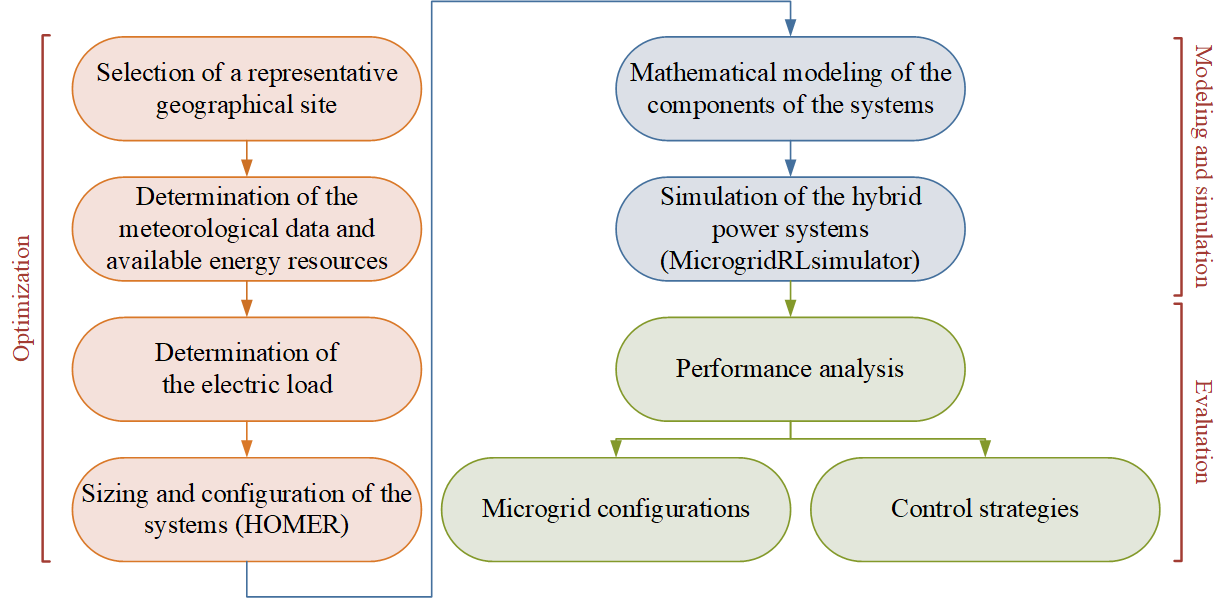
\includegraphics[scale=0.618]{Figures/Methodology.png}
    \caption{Methods and general approach of system analysis.}
    \label{fig_methods}
\end{figure}
\section{ECONOMIC OPTIMIZATION}
The following sections present a detailed description of meteorological data, load demands, components and their respective costs related to a standalone Parabolic dish-Stirling-Diesel-battery system.
\subsection{Geographical site selection}
According to the latest population and household census of Bolivia performed in 2012, the departments with the lowest electrification rate were Chuquisaca (69\%), Potosí (71\%) and Pando (72\%), where the major part of that percentages were concetrated in rural areas.\cite{InstitutoNacionaldeEstadistica2012}. The gap between urban and rural electricity access is bigger as a consequence of losses in the transmission and distribution, which affects the cost for power grid extension\cite{Branisa2016}. Consequently, a community located at Potosí department that had the most households without access to electricity was selected. Therefore, the chosen village was Pojo Pata, whose electrification rate represented less than 5\% of total households, relaying in most cases on the use of small diesel generators\cite{InstitutoNacionaldeEstadistica2012}.
\subsubsection{Geographic and demographic characteristics}
Pojo Pata is situated in Potosí Department, 42 kilometers north of its capital (-19.197, -65.744). Its average altitude above sea level is 3532 meters, that leads to a climate characterized by low temperatures \cite{VYMaps2021}. Even though, the principal economic activity is agriculture and the community has a population of 451 inhabitants and 100 households which were estimated by the year 2021\cite{InstitutoNacionaldeEstadistica2012}.
\subsection{Climatological characteristics}
This community has a high average annual solar radiation due to its location in Altiplano, which is a highland region in Bolivia. It has an estimated average direct normal solar radiation of 6.85 kWh/m$^2$/day, with variations between 5.47 kWh/m$^2$/day in winter and 8.18 kWh/m$^2$/day in summer\cite{Pfenninger2016,Gelaro2017}. Figure \ref{fig_solar_radiation_data} presents monthly average direct normal solar radiation of this community.
\begin{figure}[h!]
    \centering
    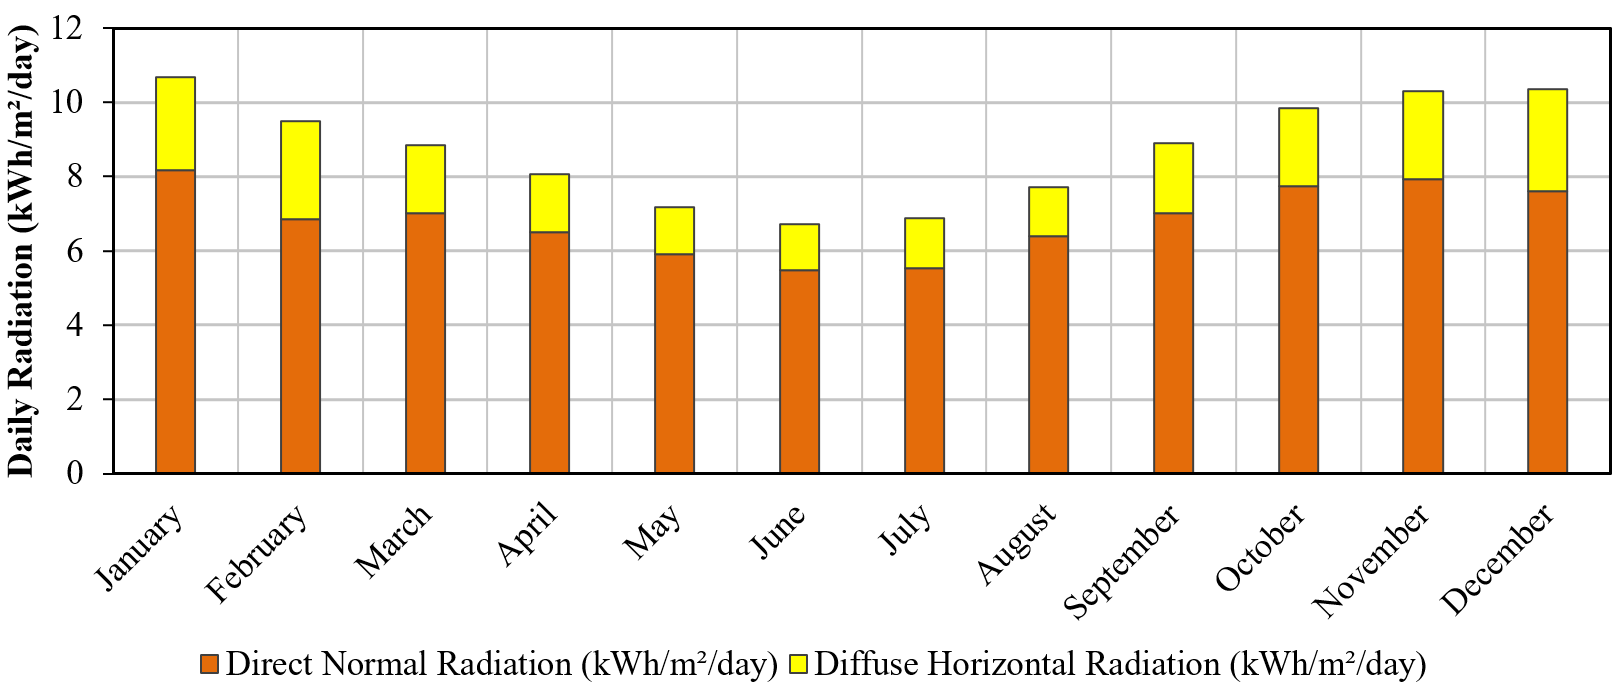
\includegraphics[scale=0.465]{Figures/Solar_radiation_data.png}
    \caption{Monthly average solar radiation data in Pojo Pata.}
    \label{fig_solar_radiation_data}
\end{figure}
%\newpage
The dry and cold climate of this community is a consequence of scarce fluvial precipitation and presence of the eastern part of Andes mountain, which act as a barrier to the flow of humid air from the Atlantic Ocean and the Amazon Basin\cite{Andressen2007}. The average annual temperature is 13.3 °C, and extreme temperatures are between 10.1 °C and 15.3 °C, in the cold and hot seasons respectively, as indicated in Figure \ref{fig_temperature_data}.
\begin{figure}[h!]
    \centering
    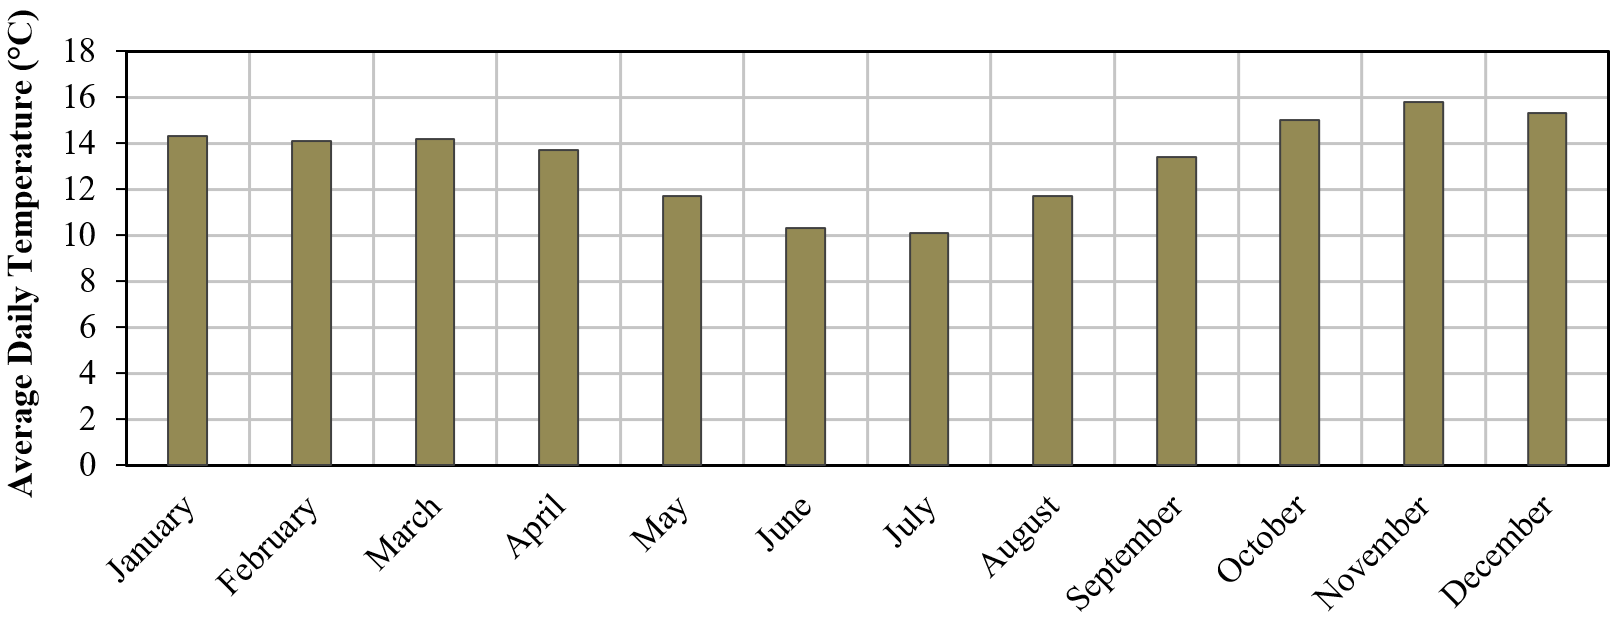
\includegraphics[scale=0.467]{Figures/Temperature_data.png}
    \caption{Monthly average temperature data in Pojo Pata.}
    \label{fig_temperature_data}
\end{figure}
\subsection{Electric energy consumption}
Pojo Pata’s electricity demand was based on 100-household located in the Altiplano zone, which is based on the demand of the community of Raqaypampa and presented in the study developed by Fernández et al.\cite{Fernandez2021}. The mentioned work contempleted villages composed of inhabitants of low and high incomes, a school, a health center, public lighting and a church. The generated daily load profiles are provided in Figure \ref{fig_electric_load}.
\begin{figure}[h!]
    \centering
    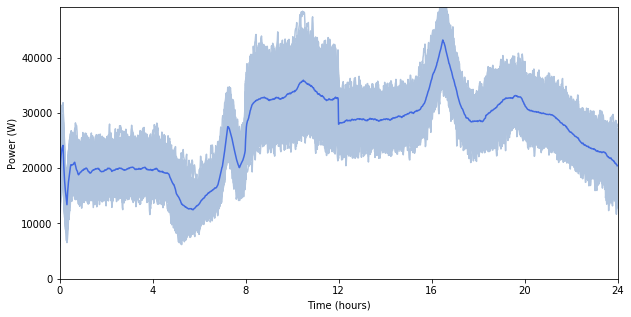
\includegraphics[scale=0.71]{Figures/Electric_load.png}
    \caption{Monthly-averaged daily load profile in Pojo Pata \cite{FernandezFuentes2020}.}
    \label{fig_electric_load}
\end{figure}
\subsection{Component specifications and inputs to HOMER}
HOMER software simulated various cases in order to find the one that would suit restrictions and the lowest net present cost (NPC). An extensive literature review was carried out in order to obtain local costs of the equipment used\cite{ENERSOLS.A.2021}. In this way, PV panel characteristics were introduced based on the technical data sheet and price of the TSM-PD14 module of TRINA SOLAR\cite{TrinaSolar2017}. Moreover, a 12 V VRLA-GEL battery (Vision CG12-200PEX) with a nominal capacity of 200 Ah was chosen\cite{ShenzhenCenterPowerTech2014} and two batteries per string were required since the electric potential of DC bus was assumed to be 24 V, according to the available technology in Bolivia. A bi-directional inverter, which has both function of a rectifier and an inverter, performed the conditioning of the system and was based on Victron MultiPlus Inverter\cite{VictronEnergy2014}.The most import parameters from diesel generator were used from the CAT C2.2 unit\cite{CaterpillarInc.2021}. Finally, the costs of PSDS system were based on the article presented by Shboul et al.\cite{Shboul2021}, that included capital cost and O\&M cost. The other parameters demanded from the aforementioned system were based on the technical characteristics of the Eurodish system, which is located in Spain and composed of a SOLO Stirling engine V161 with a maximum electrical output of 10 kW \cite{GavilanConde2011,Babikir2020}. Table \ref{Table_components} presents a summary of the characteristics of components as HOMER input data.
\begin{table}[h]
\caption{Summary of specification of components.}
\begin{center}
\resizebox{\textwidth}{!}{\begin{tabular}{c c c c c c}
\hline
Component & Size & Capital cost (USD) & Replacement cost (USD) & O\&M cost & Lifetime \\
\hline
PV Panel & 0.32 kW & 734 &	344 & 180 (USD/year) & 25 years \\
PSDS system	& 10 kW	& 28,615 &	22,710 & 576 (USD/year) & 30 years \\
Diesel genset & 1 kW & 925 & 804 & 0.0124 (USD/h) & 20,000 h \\
Battery & 200 Ah & 793 & 703 & 14 (USD/year) & 690 cycles (80\% DOD) \\
Bidirectional inverter & 1.6 kW & 1,764 & 1,604 & 160 (USD/year) & 15 years \\
\hline
\end{tabular}}
\end{center}
\label{Table_components}
\end{table}
Referred to other parameters, the lifetime of the project was taken as 20 years, the nominal discount rate was selected as 10.10\% \cite{BIDBancoInteramericanodeDesarrollo2013}, the expected inflation rate was expressed as 3.12\% \cite{BancoCentraldeBolivia2021} and the annual capacity shortage was assumed to be 0\%. The final setup of the microgrids evaluated in the software HOMER are shown in Figure \ref{fig_homer}.
\begin{figure}[h!]
    \centering
    \subfloat[PSDS-Diesel-battery system.]{\label{fig_homer_PSDS}
    \centering
    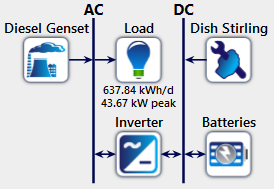
\includegraphics[width=0.4935\linewidth]{Figures/HOMER_PSDS.PNG}
    }
%no space
    \hfill
    \subfloat[PV-Diesel-battery system.]{\label{fig_homer_PV}
    \centering
    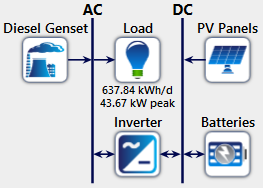
\includegraphics[width=0.478\linewidth]{Figures/HOMER_PV.PNG}
    }
    \hfill
    \subfloat[Diesel-battery system.]{\label{fig_homer_Diesel}
    \centering
    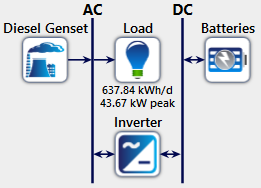
\includegraphics[width=0.48\linewidth]{Figures/HOMER_DIESEL.PNG}
    }
    \caption{HOMER architecture of microgrids.}
    \label{fig_homer}
\end{figure}
\section{MATHEMATICAL MODELING}
In this section, a detailed description of the system considered is provided (Figure \ref{fig_configuration}).The considered microgrid is composed of a solar dish Stirling engine, a Diesel genset, a battery bank, a charge controller, an inverter and a electric load. The Energy Management System (EMS) is responsible for the interaction and the scheduling of the controllable components. Therefore, the inverter and charge controller would be controlled by this one.
\begin{figure}[h!]
    \centering
    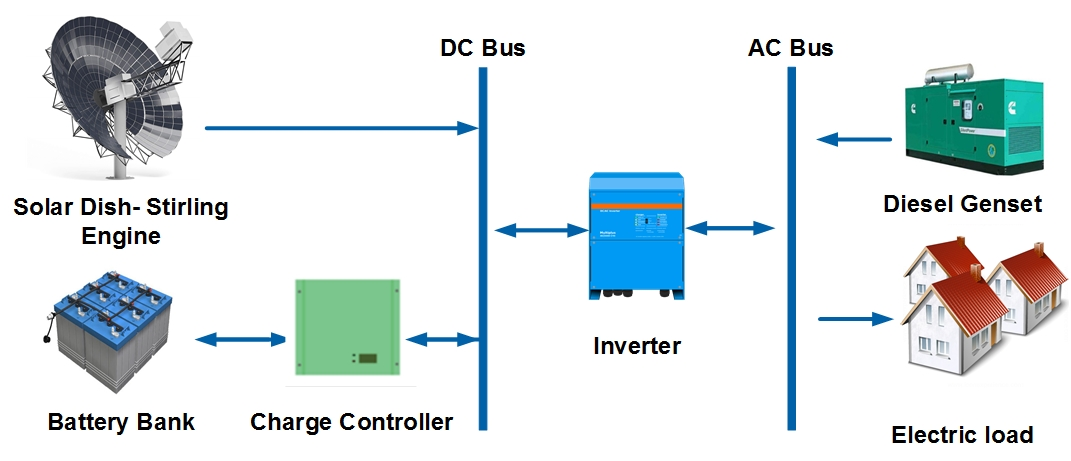
\includegraphics[scale=0.565]{Figures/Dish_Stirling_Configuration.jpg}
    \caption{Schematic diagram of the PSDS-Diesel-battery system.}
    \label{fig_configuration}
\end{figure}
\subsection{Components}
A PSDS system is composed of the following components:
\subsubsection{Consumption}
In this paper, an electric load of a rural Bolivian village (C$^{t}$) was considered non-flexible, which was related to a high cost associated to non-served energy. The demand at each time-step t was supposed to be a stochastic variable that came from distribution {$P\rlap{\textsuperscript{C}}\textsubscript{t}$}\cite{Totaro2021}.
\subsubsection{Dish-Stirling Engine}
The Dish-Stirling engine system incorporates three mainly components: Parabolic dish concentrator, solar receiver and Stirling engine coupled with an electrical generator. The direct normal radiation (DNI) is collected and reflected by the parabolic dish into the receiver, which is designed to transfer the absorbed solar energy to the working fluid in Stirling engine. The Stirling engine then converts absorbed thermal energy to mechanical power. Finally, the linear motion is converted to a rotary motion to turn a generator to generate electricity.
\subsubsection{Opto-geometric model}
The interception factor($\phi_{fi}$), which is the fraction of energy entering into the receiving cavity, could be calculated by  the following relation\cite{Bensafi2010}:
\begin{equation}
    \phi_{fi}= 1 - \exp(\frac{1}{2\cdot C\cdot {\sigma_f}^2})
\end{equation}
In this way, the lost energy outside the cavity aperture area is deduced from the interception factor.
$\sigma_{f}$ is the error of the distribution of heat flux in the focal plane, $C$ is the concentration factor defined as $C=A_{con}/A_{ap}$, where $A_{con}$ is the projected reflective surface of the solar parabolic dish concentrator and $A_{ap}$ is the aperture surface of the receiving cavity.
\subsubsection{Thermal analysis model}
The expression of the thermal power received by the aperture surface of the receiving cavity is given by the following equation \cite{Ruelas2013}.
\begin{equation}
    Q_{rec}= I\cdot A_{con}\cdot \eta_{op} \cdot\phi_{fi}
\end{equation}
Where $\eta_{op}$ is the optical efficiency of the solar parabolic dish concentrator which is defined as the product of the coefficient of absorptivity, emissivity, and transmissivity of the concentrator, $I$ is the direct normal irradiation.
In the other hand, the thermal input power to the Stirling Engine ($Q_{u}$) is estimated by subtracting the receiver thermal losses from the power intercepted by the receiver as exemplified in the equation below\cite{Rekioua2019}.
\begin{equation}
    Q_{u}= Q_{rec}-Q_{rad,ref}-(Q_{cond}+Q_{conv}+Q_{rad,emit})
    \label{Eq_SE_in}
\end{equation}
Where the terms include reflected radiation ($Q_{rad,ref}$), emitted radiation losses ($Q_{rad,emit}$), total convection losses ($Q_{conv}$), which includes both natural and forced convection, and conduction losses ($Q_{cond}$).
\subsubsection{Stirling engine}
Beale evaluated the performance of numerous Stirling engines and obtained a equation to estimate the output power, which is shown in Equation \ref{Eq_P^gross} \cite{Walker1979,Walker1980}.
\begin{equation}
    P^{gross} = B\cdot P_{m}\cdot V_{SW}\cdot f
    \label{Eq_P^gross}
\end{equation}
Here $P^{gross}$ is the gross output power of the engine, $B$ is the Beale number, $P_{m}$ is the mean engine pressure, $V_{SW}$ is the swept volume of the engine and $f$ is the engine frequency. Beale number is a parameter that characterizes the performance of Stirling engine and lies between the range from 0.11 to 0.15 for engines that function with high temperature differential\cite{Fraser2008}.
On the other hand, the net system power ($P^{net}$) is obtained by subtracting the parasitic power of the tracking motors, control system, pump, and fan from the gross output value. These parasitic losses reach an average value of 350 W during the operation of the PSDS system and a value of 10 W when the engine is off as a consequence of the uninterruptible power supply that the control system must have \cite{GavilanConde2011}.
\subsubsection{Diesel Genset}
The diesel generator operates at output level of ${P^{gen}}_t$ that is ranging between the minimum stable generation $\underline{P^{gen}}$ and the maximum capacity $\overline{P^{gen}}$ such that:
\begin{equation}
\underline{P^{gen}}\leq {P^{gen}}_t\leq\overline{P^{gen}}
\end{equation}
The fuel consumption $F_{t}$ related to the operation of the generator at time t is a function of the power output ${P^{gen}}_t$ with parameters $F_1$, $F_2$ given by the manufacturer.
\begin{equation}
F_t =
    \begin{cases}
        \text{$F_1$+$F_2\cdot{P^{gen}}_t$} & \text{,if ${P^{gen}}_t>0$,}\\
        0 & \text{,otherwise.}
    \end{cases}
\end{equation}
The fuel cost ${c^{fuel}}_t$ accounting for the fuel price $\pi^{fuel}$ is then given by:
\begin{equation}
{c^{fuel}}_t = F_t \cdot \pi^{fuel}
\end{equation}
\subsubsection{Battery bank}
The battery bank is based on a linear tank model. Therefore, the dynamics of a battery are given by the following expressions\cite{Totaro2021}:
\begin{equation}
    SOC_{t+1} = SOC_{t}+\Delta t\cdot (\eta^{ch}P^{ch}t-\frac{P^{dis}t}{\eta^{dis}})
\end{equation}
\begin{equation}
    SOC_{t},P^{ch}t,P^{dis}t\geq0
\end{equation}
\begin{equation}
    P^{ch}t\leq\overline{P}
\end{equation}
\begin{equation}
    P^{dis}t\leq\underline{P}
\end{equation}
\begin{equation}
    SOC_{t}\leq\overline{S}
\end{equation}
\begin{equation}
    \overline{S}=s(n_t)
\end{equation}
Where $SOC_t$ represents the state of charge at each time step $t$, $P^{ch}$ and $P^{dis}$ denote the charging and discharging power, respectively. Moreover, $\overline{P}$ and $\underline{P}$ are the maximum charging and discharging rates, $\overline{S}$ is the maximum battery capacity, $\eta^{ch}$ and $\eta^{dis}$ are the charging and discharging efficiencies and $n_t$ the number of cycles.
\subsubsection{Power balance}
At each time step $t$, the power balance is defined as\cite{Totaro2021}:
\begin{equation}
    {P^{net}}_t+{P^{dis}}_t+{P^{shed}}_t={P^{ch}}_t+{P^{curt}}_t+C_{t}
\end{equation}
Where $P^{shed}$ is the shedding of loads and $P^{curt}$ is the curtailment of generation.
\subsection{Control Strategies}
In this paper, two different control approaches for microgrid operation have been implemented for comparison purposes: Rule-based and optimization control.
\subsubsection{Rule-based controller}
Rule-based control strategy is simple and implements a set of rules that are taken each time step using data regarding the present state of the system. The basic principle of controller is to use the renewable generation in order to supply the electrical power demand\cite{Totaro2021}. Thus, the residual generation ($\Delta P_t$) is defined as the subtraction between the power produced from renewable resources (${P^{res}}_t$) and the demand of power ($C_t$). Thus, if there is an excess of electricity generation ($\Delta P_t>0$), then this will be used to charge the batteries. On the other hand, if the residual generation level is negative ($\Delta P_t<0$), the batteries can supply the demand. Nonetheless, prior evaluation, the actual state of charge of the batteries should be revised ($SOC$) and there are certain limits of charge ($\overline{P}$) and discharge rates ($\underline{P}$). A complete description of this algorithm is presented in Figure \ref{fig_rule_based_controller}.
\begin{figure}[h!]
    \centering
    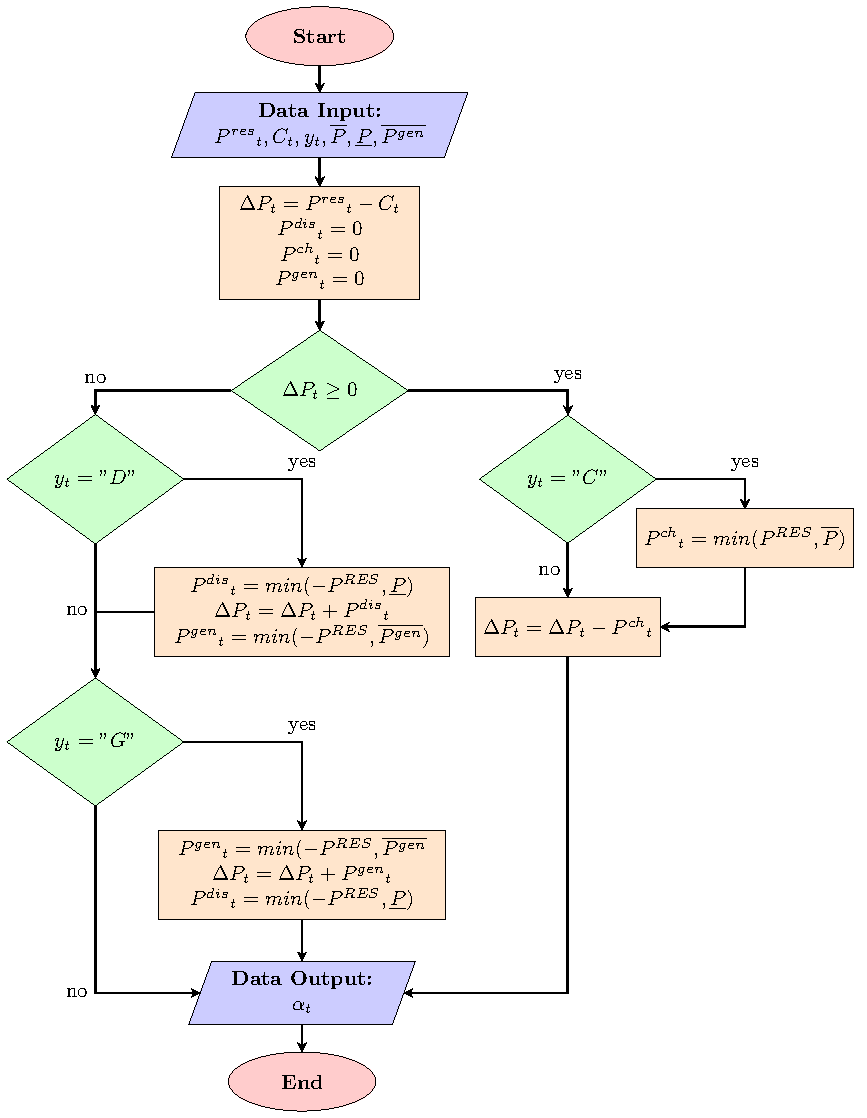
\includegraphics[scale=0.8]{Figures/Rule_based_controller.pdf}
    \caption{Flowchart of the rule-based control algorithm.}
    \label{fig_rule_based_controller}
\end{figure}
%\clearpage
\subsubsection{Optimization controller}
Optimization-based algorithms, such as the model predictive control (MPC), are not usual in today's controllers. They allow to harness optimization techniques and enable reaching multiple control objectives simultaneously. A MPC is used to establish control actions at each time step by solving an optimization problem with N-step look-ahead. In this way, the objective function tries to minimize the curtailment, load shedding and fuel cost subject to the constrains of operation which are defined by a mixed-integer linear model. Additionally, the algorithm ensures that when the genset is enabled the generation level varies between its minimum stable level and its nominal capacity\cite{Totaro2021}. The optimization problem that is solved at each current state of the system is exemplified in the flowchart in Figure \ref{fig_optimization_controller}.
\newpage
\begin{figure}[h!]
    \centering
    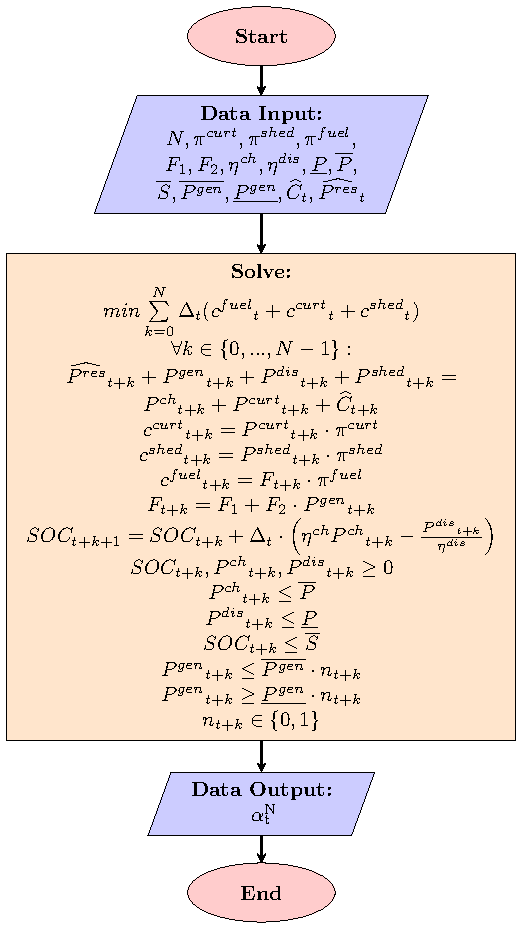
\includegraphics[scale=0.8]{Figures/Optimization controller.pdf}
    \caption{Flowchart of the optimization control algorithm.}
    \label{fig_optimization_controller}
\end{figure}
\section{RESULTS}
\subsection{Sizing}
Optimization results expressed the following microgrid configurations:
\begin{enumerate}
\item Configuration 1 (Main case) — PSDS systems (6 $\times$ 10 kW), Diesel genset (35 kW), bi-directional inverter (40 kW), and VRLA gel lead-acid battery bank (26 $\times$ 2.4 kWh).
\item Configuration 2 (Case 2) — PV panels (204 $\times$ 0.32 kW), Diesel generator (30 kW), bi-directional inverter (36 kW), and VRLA gel lead-acid battery bank (40 $\times$ 2.4 kWh). 
\item Configuration 3 (Case 3) — Diesel generator (45 kW), bi-directional inverter (0.43 kW), and VRLA gel lead-acid batteries (6 $\times$ 2.4 kWh).
\end{enumerate}
\subsection{Simulation of microgrids}
The assessment of the performance of each standalone system was developed using an open source simulator (microgridRLsimulator), which was implemented in OpenAI gym and presented by Totaro et al.\cite{Totaro2021}. This simulator envolved a complete modelling of the components of microgrids and application of any control strategy. Moreover, it requires as input data the microgrid configuration (components size, time series, and simulation parameters) and performs the simulation for a predefined simulation horizon $T$. Therefore, some important parameters used in this paper are given in Table \ref{Table_input_parameters}.
\newcolumntype{Y}{>{\centering\arraybackslash}X}
\begin{table}[h!]
\caption{Input parameters for the simulation.}
\begin{center}
\begin{threeparttable}
\begin{tabularx}{0.80\textwidth}{@{}YYY@{}}
\hline
Parameter & Value & Unit\\
\hline
$\overline{P}$,$\underline{P}$ & 0.72 & kW $\times$ battery\\
$\eta^{ch}$ & 87.65 & \%\\
$\eta^{dis}$ & 84.08 & \%\\
$\pi^{fuel}$ & 1.21 & EUR/kWh\\
$\pi^{curt}$ & 1.50 & EUR/kWh\\
$\pi^{shed}$ & 2.00 & EUR/kWh\\
$\Delta_{t}$ & 1 & h\\
\hline
\end{tabularx}
\end{threeparttable}
\label{Table_input_parameters}
\end{center}
\end{table}
\subsection{Analysis of different microgrid configurations}
In addition to evaluating the effectiveness of control strategies applied in a PSDS-Diesel-battery system, the other goal of this paper was a comparative study of the use of remote hybrid power microgrid configurations from the point of view of minimizing the operational costs.
PSDS-Diesel-battery system (Main case) was able to reduce 16\% (0.446 USD/kWh) the levelized cost of energy (LCOE) in comparison of a typical system composed of Diesel genset and a battery bank (Case 3). Nevertheless, the configuration based on PV-Diesel-battery (Case 2) represented the lowest LCOE solution (0.426 USD/kWh). According to literature, values of LCOE varies from 0.13 USD/kWh in Pakistan \cite{Lashari2021}, 0.26 USD/kWh in China \cite{Zayed2020}, 0.83 USD/kWh in Malaysia \cite{Bataineh2017} and 0.24 USD/kWh in Algeria \cite{Abbas2011} as a consequence of availability and lower local costs of technology.\\
Related to cumulative returns, Case 2 also embodied the best alternative with 55,920 EUR for an entire year. The main case and Case 3 reached 87,205 EUR and 110,259 EUR, respectively. This is shown in the graphs of Figure \ref{fig_microgrids}, which illustrate the total and accumulated costs for microgrids under a representative solar day (Winter solstice) testing period.
\begin{figure}[h!]
    \centering
    \subfloat[Main Case — PSDS-Diesel-battery system.]{\label{fig_microgrid_PSDS}
    \centering
    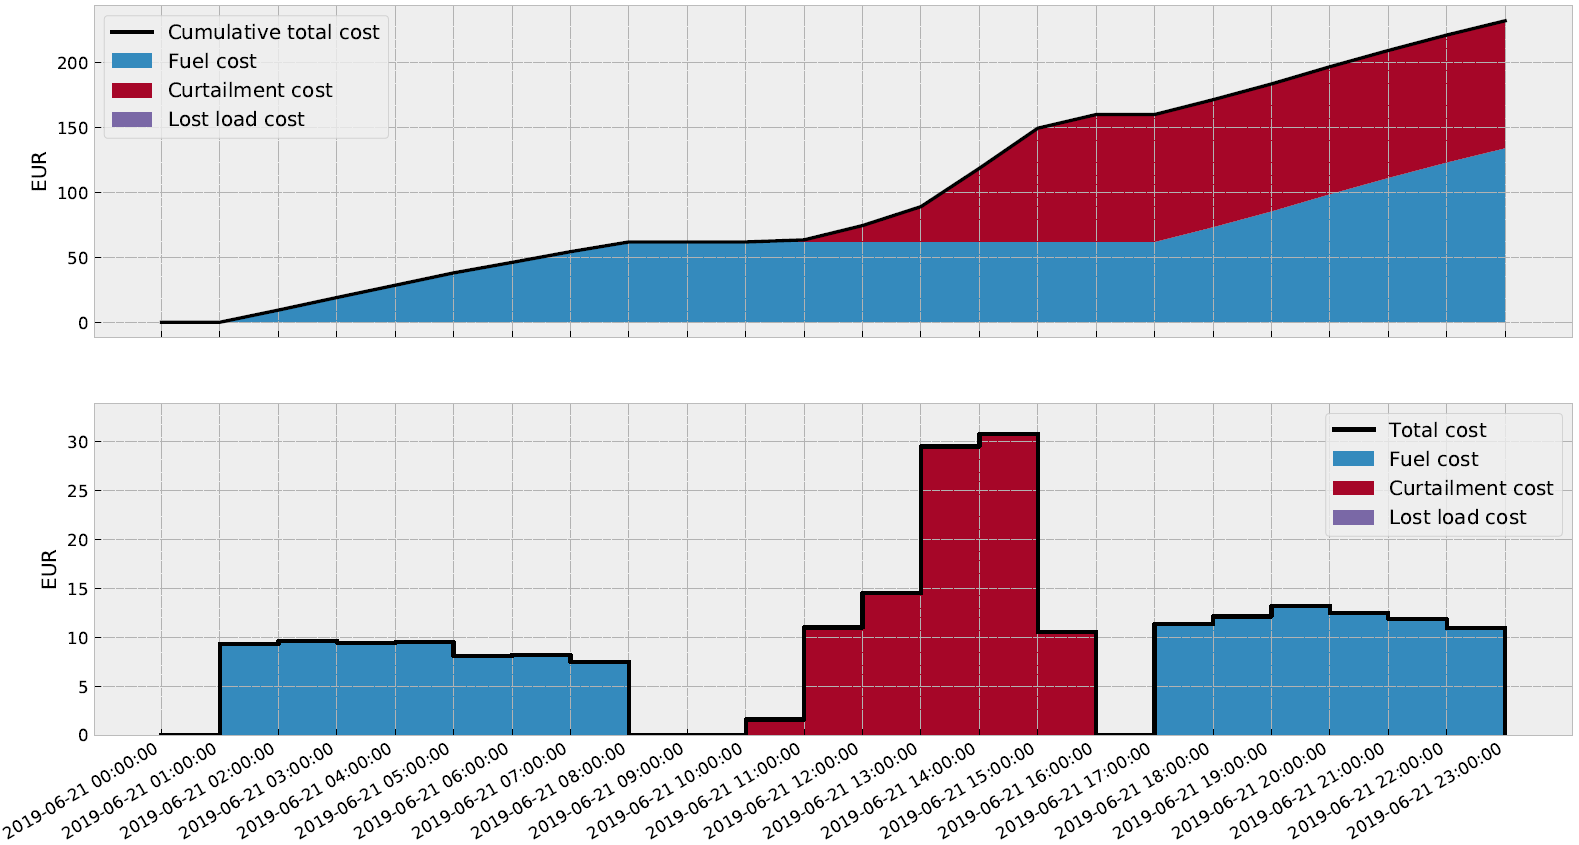
\includegraphics[scale=0.47]{Figures/Pojo_Pata_PSDS_Diesel_battery_costs.PNG}
    }
    \caption{Cumulative and total costs of the different microgrids’ configurations for winter solstice testing period.}
    \label{fig_microgrids}
\end{figure}
\begin{figure}[h!]
    \ContinuedFloat
    \centering
    \subfloat[Case 2 — PV-Diesel-battery system.]{\label{fig_microgrid_PV}
    \centering
    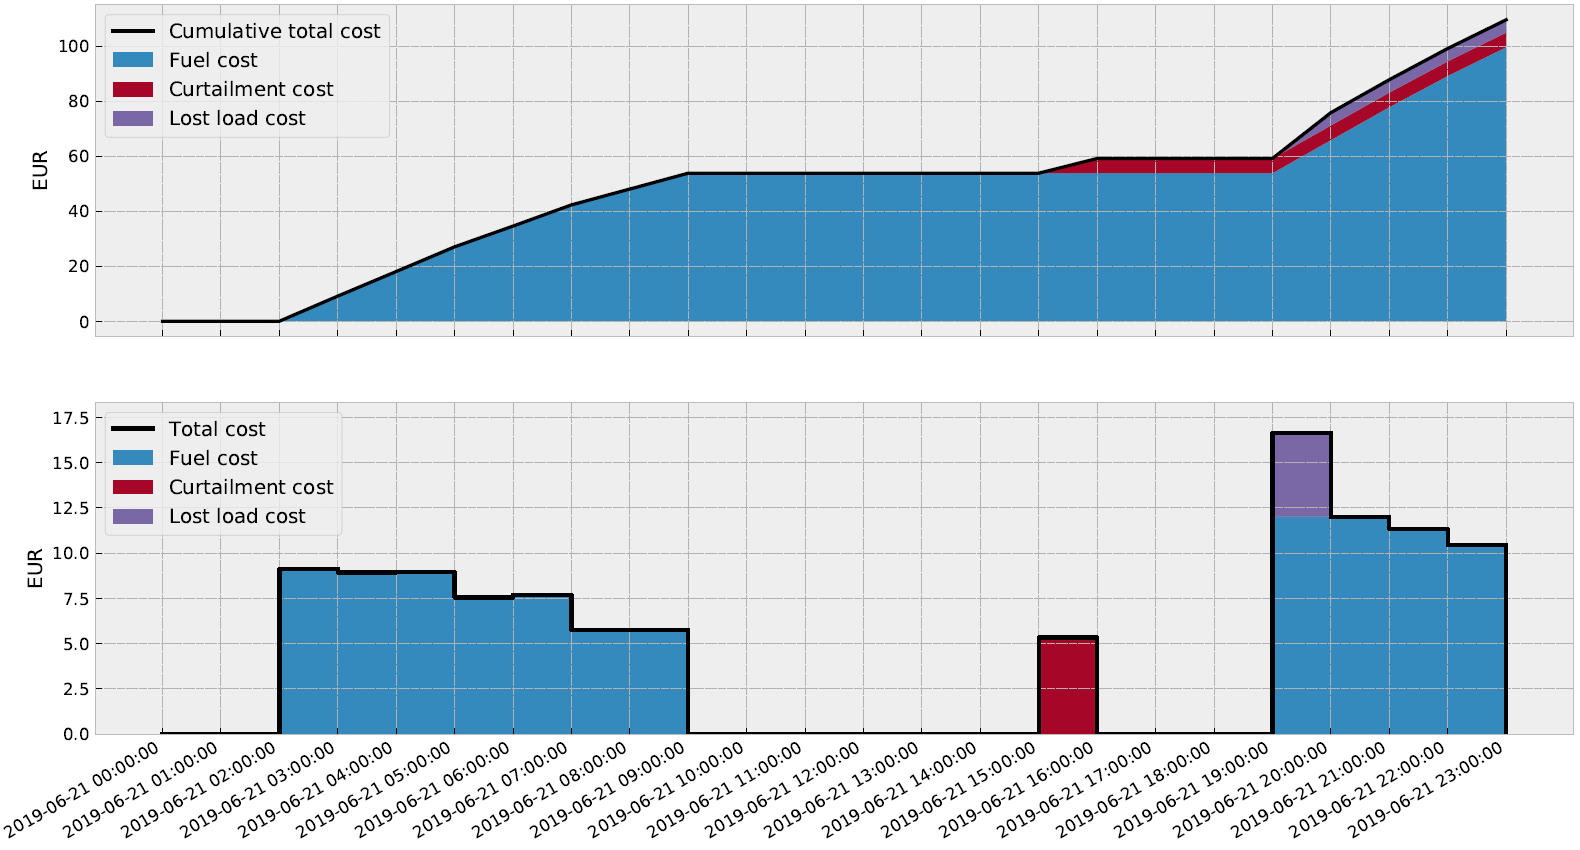
\includegraphics[scale=0.47]{Figures/Pojo_Pata_PV_Diesel_battery_costs.PNG}
    }
    \hfill
    \subfloat[Case 3 — Diesel-battery system.]{\label{fig_microgrid_Diesel}
    \centering
    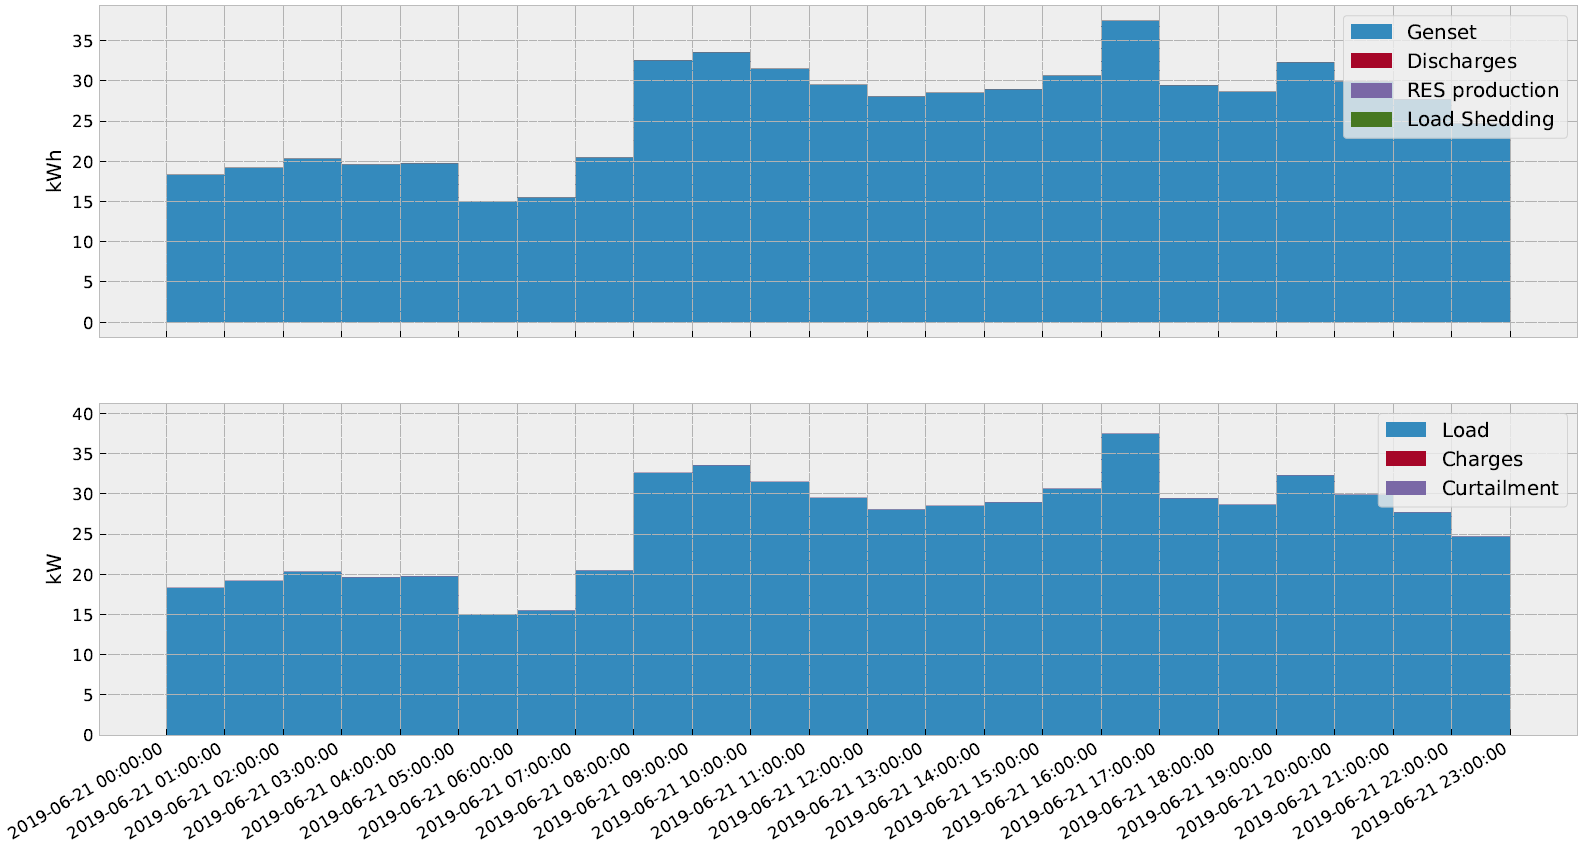
\includegraphics[scale=0.47]{Figures/Pojo_Pata_Diesel_battery_costs.PNG}
    }
    \caption{Cumulative and total costs of the different microgrids’ configurations for winter solstice testing period.}
    \label{fig_microgrids}
\end{figure}
\newpage
\subsection{Comparison between control strategies}
The rule-based controller, which is typically found in microgrid controllers nowadays, was compared against an optimization controller with perfect knowledge and 12 periods of look-ahead. In this way, the model-predictive method approximately yield a 4.25\% (83,499 EUR) for an entire year in comparison to the rule-based method. Figure \ref{fig_controllers} exemplifies the dynamics of the components of generation and consumption related to PSDS-Diesel-battery system using a rule-based algorithm and using a model-predictive algorithm during winter solstice. As it can be observed in Figures \ref{fig_rule_based_controller} and \ref{fig_optimization_controller}, the cost reduction reached is due to the less utilization of Diesel generator and the higher use of RES from the optimization algorithm.
\begin{figure}[h!]
    \centering
    \subfloat[Rule-based controller.]{\label{fig_rule_based_controller}
    \centering
    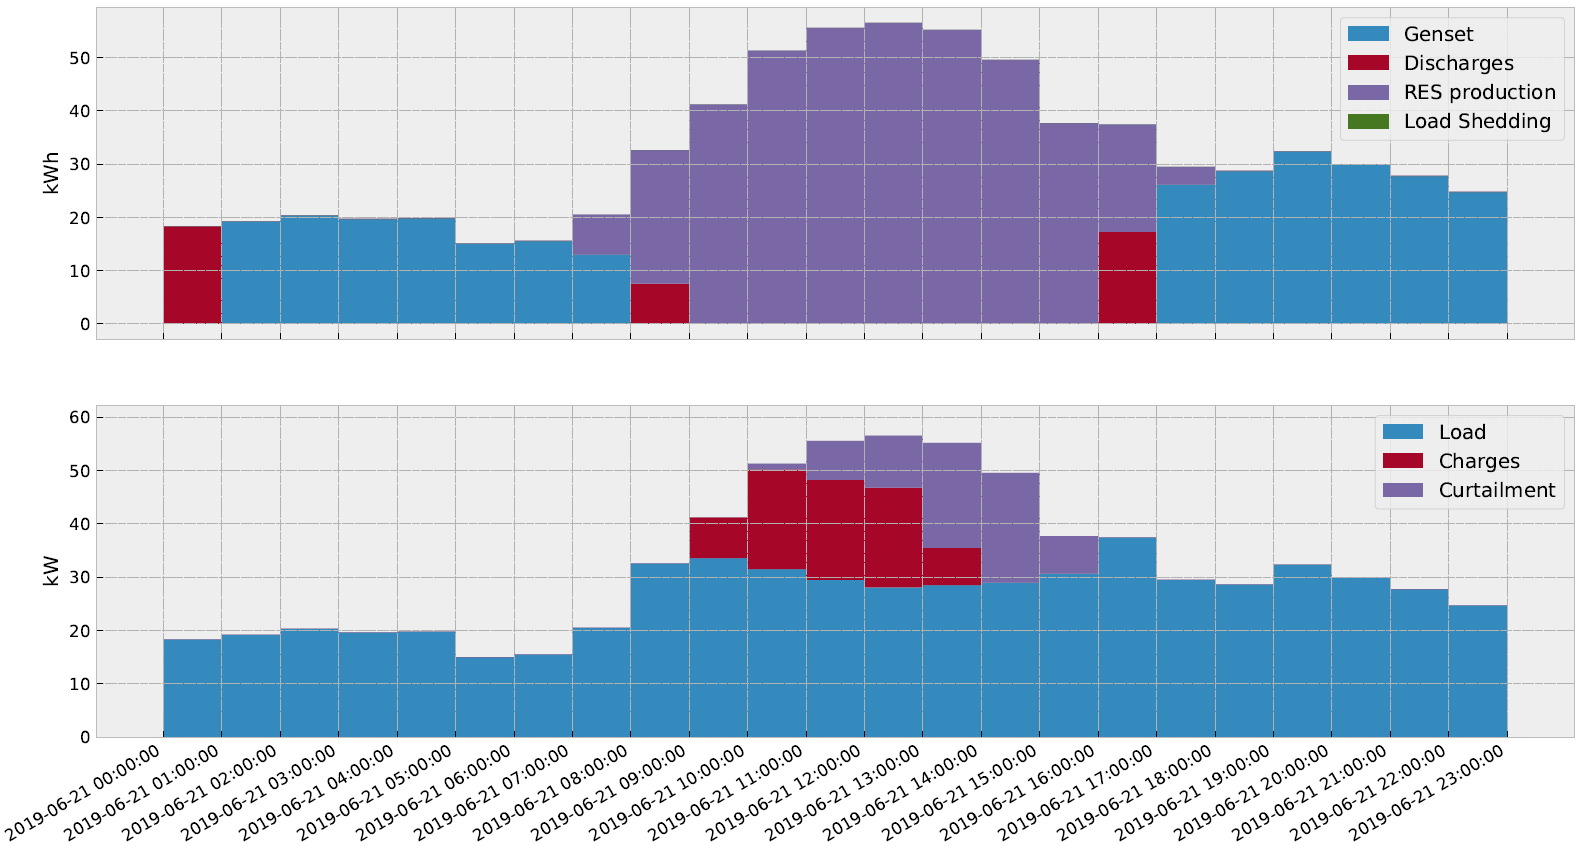
\includegraphics[scale=0.45]{Figures/RULE_BASED_CONTROLLER.PNG}
    }
    \hfill
    \subfloat[Model-predictive controller (Optimization controller).]{\label{fig_optimization_controller}
    \centering
    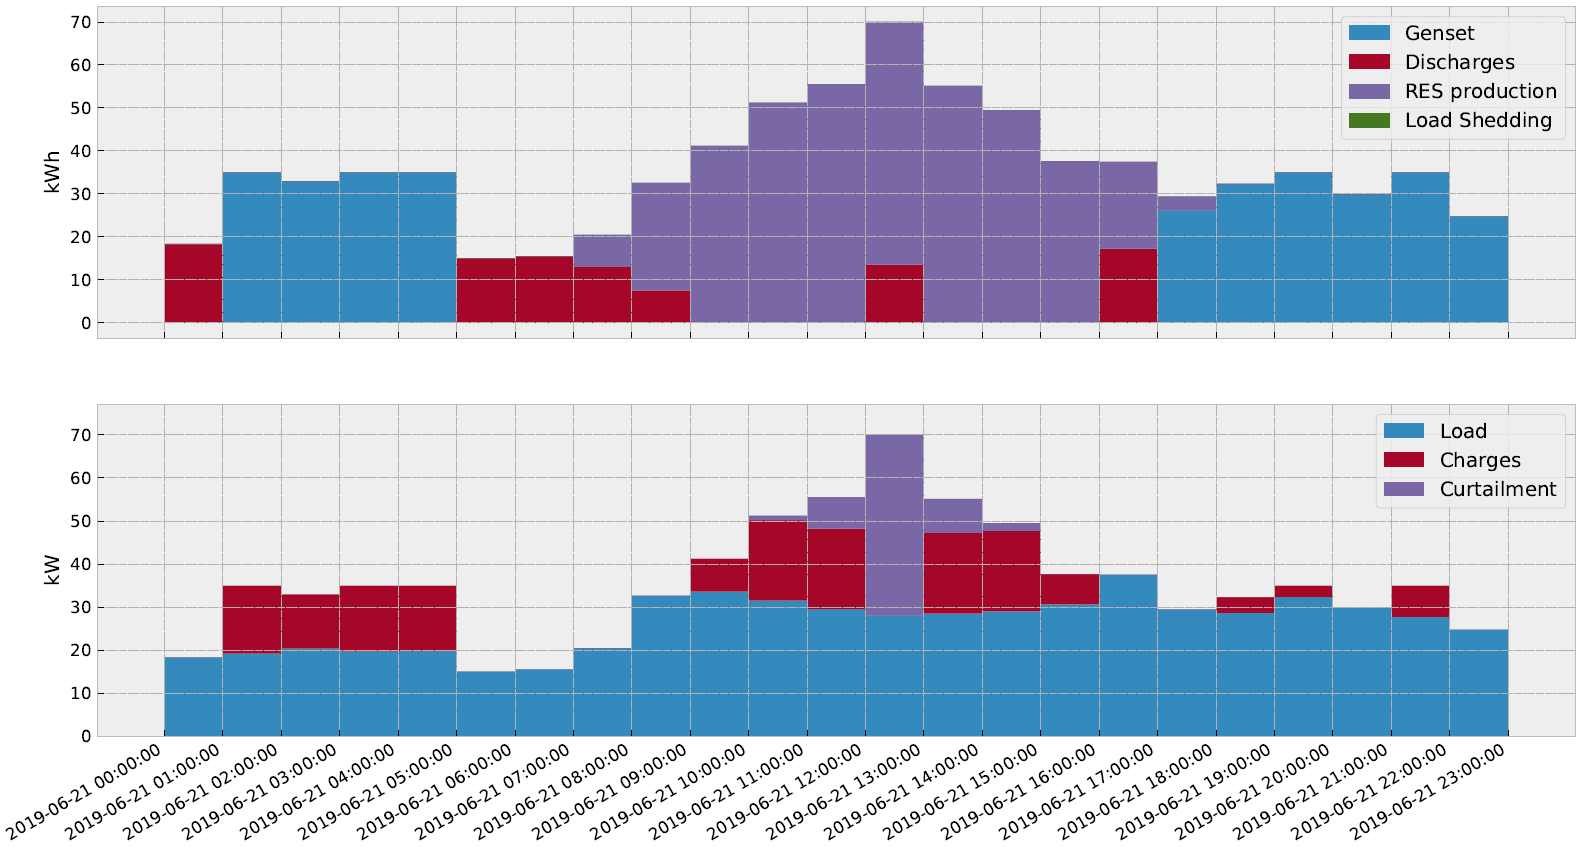
\includegraphics[scale=0.46]{Figures/OPTIMIZATION_CONTROLLER.PNG}
    }
    \caption{Generation and load mix of the PSDS-Diesel-battery system (Main case).}
    \label{fig_controllers}
\end{figure}
\\Current literature denotes that locations with a direct normal irradiation of 1800 kWh/m$^2$/year or higher have potential to install a PSDS system \cite{Thiam2017,Crespo2021}, such as the case of the studied village (2819 kWh/m$^2$/year). Despite these values are included in the range recommended, feasibility of PSDS generation systems will also depend on technology costs, project costs, and the extent of government driven financial support\cite{Stokler2016}.
\section{CONCLUSIONS}
In this paper, a comprehensive study of a novel remote hybrid microgrid (PSDS-Diesel-battery system) was presented. First, a determination of meteorological data (Solar irradiance, wind speed and average ambient temperature), techno-economic data about system components and electricity demand of the rural community of Pojo Pata was extracted in order to use that information as input for HOMER software, which led to techno-economically optimized configurations.\\
Subsequently, mathematical models were studied for the different technologies. Each model considers important factors of the evaluated technology such as the model of the Parabolic dish-Stirling engine which considered three main components involving opto-geometric and thermal characteristics.
Moreover, an open-source framework for the simulation of power grid was utilized \cite{Totaro2021}.\\
Then, a comparison between the mentioned system and other common standalone power system configurations was performed. Although the standalone PSDS-Diesel-battery system was not as cheap as the PV-Diesel-battery sytem, it represented around 21\% of operational savings in comparison to the Diesel-battery system. Additionally, the difference between LCOEs of this main case and the standalone hybrid solar system was minimal.\\
Finally, an assessment of two different control strategies for the Main case was performed. The model-predictive controller was able to outperform the common rule-based controller, as it reached near 4\% of savings.
Besides the high purchase price of the Stirling engine and its unavailability in the Bolivian market, the hybrid system based on a parabolic dish, Stirling engine and batteries for the community of Pojo Pata represented a better option to implement in a rural electrification project compared to a system made up of Diesel generator and batteries. There is a great opportunity for systems based on Stirling engines to benefit users of distributed energy systems, as the technology matures, and more developments are made in the energy field. Moreover, the policy measures are required to rise the financial attraction and decrease the investment costs of PSDS systems for the competitiveness with other concentrated solar power technologies.
\newpage
\nomenclature[V]{\(C_{t}\)}{Electric load at each time-step $t$ (kW)}
\nomenclature[F]{\(P\rlap{\textsuperscript{C}}\textsubscript{t}\)}{Load probability distribution}
\nomenclature[P]{\(\phi_{fi}\)}{Interception factor}
\nomenclature[P]{\(C\)}{Concentration factor}
\nomenclature[P]{\(\sigma_{f}\)}{Error of the distribution of heat flux in the focal plane}
\nomenclature[P]{\(A_{con}\)}{Projected reflective surface of parabolic dish (m$^2$)}
\nomenclature[P]{\(A_{ap}\)}{Aperture surface of receiving cavity (m$^2$)}
\nomenclature[V]{\(Q_{rec}\)}{Thermal power at receiving cavity (W)}
\nomenclature[P]{\(\eta_{op}\)}{Optical efficiency of parabolic dish concentrator}
\nomenclature[V]{\(I\)}{Direct Normal Irradiation(W/m$^2$)}
\nomenclature[V]{\(Q_{u}\)}{Thermal input power to the Stirling Engine (W)}
\nomenclature[V]{\(Q_{rad,ref}\)}{Reflected radiation losses (W)}
\nomenclature[V]{\(Q_{rad,emit}\)}{Emitted radiation losses (W)}
\nomenclature[V]{\(Q_{conv}\)}{Convection losses (W)}
\nomenclature[V]{\(Q_{cond}\)}{Conduction losses (W)}
\nomenclature[P]{\(B\)}{Beale number}
\nomenclature[P]{\(P_{m}\)}{Mean Stirling engine pressure (Pa)}
\nomenclature[P]{\(V_{SW}\)}{Displaced Stirling engine volume (m$^3$)}
\nomenclature[P]{\(f\)}{Stirling engine frequency (Hz)}
\nomenclature[V]{\(P^{gross}\)}{Gross output power of Stirling engine (W)}
\nomenclature[V]{\(P^{net}\)}{Net output power of Stirling engine (kW)}
\nomenclature[V]{\({P^{gen}}_t\)}{Power output of Diesel genset (kW)}
\nomenclature[P]{\(\underline{P^{gen}}\)}{Minimum stable generation of Diesel genset (kW)}
\nomenclature[P]{\(\overline{P^{gen}}\)}{Maximum capacity of Diesel genset (kW)}
\nomenclature[V]{\(F_t\)}{Fuel consumption of diesel genset (l)}
\nomenclature[P]{\(F_1\)}{Fuel consumption parameter of diesel genset}
\nomenclature[P]{\(F_2\)}{Fuel consumption parameter of diesel genset}
\nomenclature[V]{\({c^{fuel}}_t\)}{Fuel cost (EUR)}
\nomenclature[P]{\(\pi^{fuel}\)}{Fuel price (EUR/kWh)}
\nomenclature[P]{\(\eta_{gen}\)}{Electrical efficiency of generator}
\nomenclature[V]{\(SOC_t\)}{State of charge of battery bank at each time step (kWh)}
\nomenclature[V]{\(SOC_{t+1}\)}{State of charge of battery bank at next time step (kWh)}
\nomenclature[V]{\(P^{ch}\)}{Charging power of battery bank (kWh)}
\nomenclature[V]{\(P^{dis}\)}{Discharging power of battery bank (kWh)}
\nomenclature[P]{\(\overline{P}\)}{Maximum charging rate of battery bank (kW)}
\nomenclature[P]{\(\underline{P}\)}{Maximum discharging rate of battery bank (kW)}
\nomenclature[P]{\(\overline{S}\)}{Maximum battery capacity (kWh)}
\nomenclature[P]{\(\eta^{ch}\)}{Charging efficiency of battery bank}
\nomenclature[P]{\(\eta^{dis}\)}{Discharging efficiency of battery bank}
\nomenclature[V]{\(n_t\)}{Number of cycles of battery}
\nomenclature[V]{\({P^{shed}}_t\)}{Shedding of loads (kW)}
\nomenclature[V]{\({P^{curt}}_t\)}{Curtailment of generation (kW)}
\nomenclature[V]{\({P^{res}}_t\)}{Renewable generation (PSDS or PV panels) (kW)}
\nomenclature[V]{\(y_t\)}{Discrete decision about the use of the equipment}
\nomenclature[V]{\(\Delta P_t\)}{Residual generation level (kW)}
\nomenclature[V]{\(\alpha_t\)}{Control actions vector}
\nomenclature[P]{\(N\)}{Number of look-ahead periods}
\nomenclature[P]{\(\pi^{curt}\)}{Curtailment price (EUR/kWh)}
\nomenclature[P]{\(\pi^{shed}\)}{Load shedding price (EUR/kWh)}
\nomenclature[P]{\(\widehat{C}\)}{Load forecast (kW)}
\nomenclature[P]{\(\widehat{P^{res}}\)}{Renewable generation forecast (kW)}
\nomenclature[V]{\(c^{fuel}\)}{Fuel cost (EUR)}
\nomenclature[V]{\(c^{curt}\)}{Curtailment cost (EUR)}
\nomenclature[V]{\(c^{shed}\)}{Lost load cost (EUR)}
\nomenclature[P]{\(\Delta_t\)}{Simulation and control period duration (h)}
\nomenclature[S]{\(t\)}{Decision time step}
\nomenclature[S]{\(k\)}{Look-ahead step}
\printnomenclature
\newpage
\bibliographystyle{ieeetr}
\bibliography{Solar_Stirling}
\end{document}